% AUTO-GENERATED by fhlm/make_paper_tables.py from main.tex -- edit main.tex, not this file.
\documentclass[conference]{IEEEtran}
\IEEEoverridecommandlockouts
\usepackage{cite}
\usepackage{amsmath,amssymb,amsfonts,amsthm}
\usepackage{algorithmic}
\usepackage{algorithm}
\usepackage{graphicx}
\usepackage{textcomp}
\usepackage{xcolor}
\usepackage{booktabs}
\usepackage{url}
\graphicspath{{figures/}}
% ---- inlined from generated/macros ----
\newcommand{\nSeeds}{20}
\newcommand{\nRuns}{1000}
\newcommand{\nMethods}{10}
\newcommand{\meanlowstaticequal}{4.45}
\newcommand{\meanlowstaticequalLL}{1.3}
\newcommand{\meanlowstaticequalEMBB}{7.4}
\newcommand{\meanlowstaticequalUtil}{47.2}
\newcommand{\meanlowreactiveprop}{0.83}
\newcommand{\meanlowreactivepropLL}{1.6}
\newcommand{\meanlowreactivepropEMBB}{0.1}
\newcommand{\meanlowreactivepropUtil}{50.0}
\newcommand{\meanlowmaxweight}{0.90}
\newcommand{\meanlowmaxweightLL}{1.8}
\newcommand{\meanlowmaxweightEMBB}{0.1}
\newcommand{\meanlowmaxweightUtil}{50.0}
\newcommand{\meanlowqueueaware}{0.52}
\newcommand{\meanlowqueueawareLL}{0.7}
\newcommand{\meanlowqueueawareEMBB}{0.3}
\newcommand{\meanlowqueueawareUtil}{50.0}
\newcommand{\meanlowpointforecast}{0.27}
\newcommand{\meanlowpointforecastLL}{0.3}
\newcommand{\meanlowpointforecastEMBB}{0.2}
\newcommand{\meanlowpointforecastUtil}{50.1}
\newcommand{\meanlowfixedquantile}{0.34}
\newcommand{\meanlowfixedquantileLL}{0.1}
\newcommand{\meanlowfixedquantileEMBB}{0.5}
\newcommand{\meanlowfixedquantileUtil}{50.0}
\newcommand{\meanlowproposedwindow}{0.25}
\newcommand{\meanlowproposedwindowLL}{0.4}
\newcommand{\meanlowproposedwindowEMBB}{0.1}
\newcommand{\meanlowproposedwindowUtil}{50.1}
\newcommand{\meanlowproposed}{0.15}
\newcommand{\meanlowproposedLL}{0.2}
\newcommand{\meanlowproposedEMBB}{0.1}
\newcommand{\meanlowproposedUtil}{50.1}
\newcommand{\meanlowproposedcal}{0.17}
\newcommand{\meanlowproposedcalLL}{0.2}
\newcommand{\meanlowproposedcalEMBB}{0.1}
\newcommand{\meanlowproposedcalUtil}{50.1}
\newcommand{\meanloworacle}{0.07}
\newcommand{\meanloworacleLL}{0.0}
\newcommand{\meanloworacleEMBB}{0.1}
\newcommand{\meanloworacleUtil}{50.2}
\newcommand{\meanmoderatestaticequal}{9.65}
\newcommand{\meanmoderatestaticequalLL}{4.8}
\newcommand{\meanmoderatestaticequalEMBB}{14.2}
\newcommand{\meanmoderatestaticequalUtil}{57.5}
\newcommand{\meanmoderatereactiveprop}{4.11}
\newcommand{\meanmoderatereactivepropLL}{7.6}
\newcommand{\meanmoderatereactivepropEMBB}{0.8}
\newcommand{\meanmoderatereactivepropUtil}{63.5}
\newcommand{\meanmoderatemaxweight}{4.85}
\newcommand{\meanmoderatemaxweightLL}{9.3}
\newcommand{\meanmoderatemaxweightEMBB}{0.7}
\newcommand{\meanmoderatemaxweightUtil}{63.3}
\newcommand{\meanmoderatequeueaware}{4.24}
\newcommand{\meanmoderatequeueawareLL}{3.3}
\newcommand{\meanmoderatequeueawareEMBB}{5.1}
\newcommand{\meanmoderatequeueawareUtil}{62.2}
\newcommand{\meanmoderatepointforecast}{3.23}
\newcommand{\meanmoderatepointforecastLL}{1.8}
\newcommand{\meanmoderatepointforecastEMBB}{4.6}
\newcommand{\meanmoderatepointforecastUtil}{62.7}
\newcommand{\meanmoderatefixedquantile}{4.35}
\newcommand{\meanmoderatefixedquantileLL}{0.6}
\newcommand{\meanmoderatefixedquantileEMBB}{7.9}
\newcommand{\meanmoderatefixedquantileUtil}{61.3}
\newcommand{\meanmoderateproposedwindow}{2.57}
\newcommand{\meanmoderateproposedwindowLL}{2.0}
\newcommand{\meanmoderateproposedwindowEMBB}{3.1}
\newcommand{\meanmoderateproposedwindowUtil}{63.4}
\newcommand{\meanmoderateproposed}{2.15}
\newcommand{\meanmoderateproposedLL}{1.4}
\newcommand{\meanmoderateproposedEMBB}{2.8}
\newcommand{\meanmoderateproposedUtil}{63.6}
\newcommand{\meanmoderateproposedcal}{2.17}
\newcommand{\meanmoderateproposedcalLL}{1.4}
\newcommand{\meanmoderateproposedcalEMBB}{2.9}
\newcommand{\meanmoderateproposedcalUtil}{63.6}
\newcommand{\meanmoderateoracle}{1.62}
\newcommand{\meanmoderateoracleLL}{0.0}
\newcommand{\meanmoderateoracleEMBB}{3.1}
\newcommand{\meanmoderateoracleUtil}{63.7}
\newcommand{\meanhighstaticequal}{15.46}
\newcommand{\meanhighstaticequalLL}{9.8}
\newcommand{\meanhighstaticequalEMBB}{20.8}
\newcommand{\meanhighstaticequalUtil}{65.8}
\newcommand{\meanhighreactiveprop}{9.20}
\newcommand{\meanhighreactivepropLL}{14.7}
\newcommand{\meanhighreactivepropEMBB}{4.0}
\newcommand{\meanhighreactivepropUtil}{74.7}
\newcommand{\meanhighmaxweight}{11.54}
\newcommand{\meanhighmaxweightLL}{20.6}
\newcommand{\meanhighmaxweightEMBB}{2.9}
\newcommand{\meanhighmaxweightUtil}{74.1}
\newcommand{\meanhighqueueaware}{11.03}
\newcommand{\meanhighqueueawareLL}{5.2}
\newcommand{\meanhighqueueawareEMBB}{16.5}
\newcommand{\meanhighqueueawareUtil}{69.3}
\newcommand{\meanhighpointforecast}{9.70}
\newcommand{\meanhighpointforecastLL}{3.1}
\newcommand{\meanhighpointforecastEMBB}{16.0}
\newcommand{\meanhighpointforecastUtil}{70.1}
\newcommand{\meanhighfixedquantile}{11.76}
\newcommand{\meanhighfixedquantileLL}{0.9}
\newcommand{\meanhighfixedquantileEMBB}{22.0}
\newcommand{\meanhighfixedquantileUtil}{67.0}
\newcommand{\meanhighproposedwindow}{8.72}
\newcommand{\meanhighproposedwindowLL}{3.7}
\newcommand{\meanhighproposedwindowEMBB}{13.5}
\newcommand{\meanhighproposedwindowUtil}{71.5}
\newcommand{\meanhighproposed}{8.00}
\newcommand{\meanhighproposedLL}{3.4}
\newcommand{\meanhighproposedEMBB}{12.3}
\newcommand{\meanhighproposedUtil}{72.2}
\newcommand{\meanhighproposedcal}{8.14}
\newcommand{\meanhighproposedcalLL}{2.9}
\newcommand{\meanhighproposedcalEMBB}{13.1}
\newcommand{\meanhighproposedcalUtil}{71.9}
\newcommand{\meanhighoracle}{6.89}
\newcommand{\meanhighoracleLL}{0.0}
\newcommand{\meanhighoracleEMBB}{13.4}
\newcommand{\meanhighoracleUtil}{72.3}
\newcommand{\meanoverloadburstsstaticequal}{19.15}
\newcommand{\meanoverloadburstsstaticequalLL}{13.4}
\newcommand{\meanoverloadburstsstaticequalEMBB}{24.2}
\newcommand{\meanoverloadburstsstaticequalUtil}{67.9}
\newcommand{\meanoverloadburstsreactiveprop}{12.27}
\newcommand{\meanoverloadburstsreactivepropLL}{17.8}
\newcommand{\meanoverloadburstsreactivepropEMBB}{7.1}
\newcommand{\meanoverloadburstsreactivepropUtil}{78.0}
\newcommand{\meanoverloadburstsmaxweight}{15.24}
\newcommand{\meanoverloadburstsmaxweightLL}{25.4}
\newcommand{\meanoverloadburstsmaxweightEMBB}{5.8}
\newcommand{\meanoverloadburstsmaxweightUtil}{77.0}
\newcommand{\meanoverloadburstsqueueaware}{14.51}
\newcommand{\meanoverloadburstsqueueawareLL}{6.2}
\newcommand{\meanoverloadburstsqueueawareEMBB}{22.1}
\newcommand{\meanoverloadburstsqueueawareUtil}{71.0}
\newcommand{\meanoverloadburstspointforecast}{13.33}
\newcommand{\meanoverloadburstspointforecastLL}{4.1}
\newcommand{\meanoverloadburstspointforecastEMBB}{21.8}
\newcommand{\meanoverloadburstspointforecastUtil}{71.7}
\newcommand{\meanoverloadburstsfixedquantile}{15.09}
\newcommand{\meanoverloadburstsfixedquantileLL}{1.9}
\newcommand{\meanoverloadburstsfixedquantileEMBB}{27.3}
\newcommand{\meanoverloadburstsfixedquantileUtil}{68.7}
\newcommand{\meanoverloadburstsproposedwindow}{12.67}
\newcommand{\meanoverloadburstsproposedwindowLL}{4.4}
\newcommand{\meanoverloadburstsproposedwindowEMBB}{20.3}
\newcommand{\meanoverloadburstsproposedwindowUtil}{72.6}
\newcommand{\meanoverloadburstsproposed}{11.76}
\newcommand{\meanoverloadburstsproposedLL}{4.6}
\newcommand{\meanoverloadburstsproposedEMBB}{18.3}
\newcommand{\meanoverloadburstsproposedUtil}{73.8}
\newcommand{\meanoverloadburstsproposedcal}{12.27}
\newcommand{\meanoverloadburstsproposedcalLL}{3.6}
\newcommand{\meanoverloadburstsproposedcalEMBB}{20.3}
\newcommand{\meanoverloadburstsproposedcalUtil}{72.8}
\newcommand{\meanoverloadburstsoracle}{10.16}
\newcommand{\meanoverloadburstsoracleLL}{0.4}
\newcommand{\meanoverloadburstsoracleEMBB}{19.1}
\newcommand{\meanoverloadburstsoracleUtil}{74.3}
\newcommand{\meanshiftstaticequal}{22.31}
\newcommand{\meanshiftstaticequalLL}{19.0}
\newcommand{\meanshiftstaticequalEMBB}{25.2}
\newcommand{\meanshiftstaticequalUtil}{54.5}
\newcommand{\meanshiftreactiveprop}{11.70}
\newcommand{\meanshiftreactivepropLL}{14.4}
\newcommand{\meanshiftreactivepropEMBB}{9.0}
\newcommand{\meanshiftreactivepropUtil}{64.0}
\newcommand{\meanshiftmaxweight}{12.31}
\newcommand{\meanshiftmaxweightLL}{16.5}
\newcommand{\meanshiftmaxweightEMBB}{8.2}
\newcommand{\meanshiftmaxweightUtil}{64.0}
\newcommand{\meanshiftqueueaware}{12.56}
\newcommand{\meanshiftqueueawareLL}{10.5}
\newcommand{\meanshiftqueueawareEMBB}{14.4}
\newcommand{\meanshiftqueueawareUtil}{61.9}
\newcommand{\meanshiftpointforecast}{11.30}
\newcommand{\meanshiftpointforecastLL}{7.8}
\newcommand{\meanshiftpointforecastEMBB}{14.6}
\newcommand{\meanshiftpointforecastUtil}{62.3}
\newcommand{\meanshiftfixedquantile}{12.85}
\newcommand{\meanshiftfixedquantileLL}{5.0}
\newcommand{\meanshiftfixedquantileEMBB}{20.2}
\newcommand{\meanshiftfixedquantileUtil}{59.9}
\newcommand{\meanshiftproposedwindow}{10.22}
\newcommand{\meanshiftproposedwindowLL}{6.1}
\newcommand{\meanshiftproposedwindowEMBB}{14.1}
\newcommand{\meanshiftproposedwindowUtil}{62.9}
\newcommand{\meanshiftproposed}{10.04}
\newcommand{\meanshiftproposedLL}{6.6}
\newcommand{\meanshiftproposedEMBB}{13.2}
\newcommand{\meanshiftproposedUtil}{63.3}
\newcommand{\meanshiftproposedcal}{11.12}
\newcommand{\meanshiftproposedcalLL}{4.7}
\newcommand{\meanshiftproposedcalEMBB}{17.2}
\newcommand{\meanshiftproposedcalUtil}{61.5}
\newcommand{\meanshiftoracle}{6.69}
\newcommand{\meanshiftoracleLL}{0.9}
\newcommand{\meanshiftoracleEMBB}{12.1}
\newcommand{\meanshiftoracleUtil}{65.0}
\newcommand{\redhighstaticequal}{48}
\newcommand{\redhighstaticequalWins}{20/20}
\newcommand{\redhighstaticequalP}{0.000}
\newcommand{\redhighstaticequalCI}{[46, 50]}
\newcommand{\redhighreactiveprop}{13}
\newcommand{\redhighreactivepropWins}{20/20}
\newcommand{\redhighreactivepropP}{0.000}
\newcommand{\redhighreactivepropCI}{[11, 16]}
\newcommand{\redhighmaxweight}{31}
\newcommand{\redhighmaxweightWins}{20/20}
\newcommand{\redhighmaxweightP}{0.000}
\newcommand{\redhighmaxweightCI}{[29, 33]}
\newcommand{\redhighqueueaware}{27}
\newcommand{\redhighqueueawareWins}{20/20}
\newcommand{\redhighqueueawareP}{0.000}
\newcommand{\redhighqueueawareCI}{[26, 29]}
\newcommand{\redhighpointforecast}{18}
\newcommand{\redhighpointforecastWins}{20/20}
\newcommand{\redhighpointforecastP}{0.000}
\newcommand{\redhighpointforecastCI}{[17, 19]}
\newcommand{\redhighfixedquantile}{32}
\newcommand{\redhighfixedquantileWins}{20/20}
\newcommand{\redhighfixedquantileP}{0.000}
\newcommand{\redhighfixedquantileCI}{[31, 33]}
\newcommand{\redhighproposedwindow}{8}
\newcommand{\redhighproposedwindowWins}{20/20}
\newcommand{\redhighproposedwindowP}{0.000}
\newcommand{\redhighproposedwindowCI}{[8, 9]}
\newcommand{\redhighproposedcal}{2}
\newcommand{\redhighproposedcalWins}{19/20}
\newcommand{\redhighproposedcalP}{0.000}
\newcommand{\redhighproposedcalCI}{[1, 2]}
\newcommand{\redhighoracle}{-16}
\newcommand{\redhighoracleWins}{0/20}
\newcommand{\redhighoracleP}{0.000}
\newcommand{\redhighoracleCI}{[-18, -14]}
\newcommand{\redlowstaticequal}{97}
\newcommand{\redlowstaticequalWins}{20/20}
\newcommand{\redlowstaticequalP}{0.000}
\newcommand{\redlowstaticequalCI}{[95, 98]}
\newcommand{\redlowreactiveprop}{81}
\newcommand{\redlowreactivepropWins}{20/20}
\newcommand{\redlowreactivepropP}{0.000}
\newcommand{\redlowreactivepropCI}{[75, 87]}
\newcommand{\redlowmaxweight}{83}
\newcommand{\redlowmaxweightWins}{20/20}
\newcommand{\redlowmaxweightP}{0.000}
\newcommand{\redlowmaxweightCI}{[77, 88]}
\newcommand{\redlowqueueaware}{70}
\newcommand{\redlowqueueawareWins}{20/20}
\newcommand{\redlowqueueawareP}{0.000}
\newcommand{\redlowqueueawareCI}{[62, 77]}
\newcommand{\redlowpointforecast}{43}
\newcommand{\redlowpointforecastWins}{20/20}
\newcommand{\redlowpointforecastP}{0.000}
\newcommand{\redlowpointforecastCI}{[33, 52]}
\newcommand{\redlowfixedquantile}{54}
\newcommand{\redlowfixedquantileWins}{20/20}
\newcommand{\redlowfixedquantileP}{0.000}
\newcommand{\redlowfixedquantileCI}{[44, 63]}
\newcommand{\redlowproposedwindow}{37}
\newcommand{\redlowproposedwindowWins}{20/20}
\newcommand{\redlowproposedwindowP}{0.000}
\newcommand{\redlowproposedwindowCI}{[29, 47]}
\newcommand{\redlowproposedcal}{9}
\newcommand{\redlowproposedcalWins}{18/20}
\newcommand{\redlowproposedcalP}{0.000}
\newcommand{\redlowproposedcalCI}{[5, 15]}
\newcommand{\redloworacle}{-130}
\newcommand{\redloworacleWins}{0/20}
\newcommand{\redloworacleP}{0.000}
\newcommand{\redloworacleCI}{[-288, -78]}
\newcommand{\redmoderatestaticequal}{78}
\newcommand{\redmoderatestaticequalWins}{20/20}
\newcommand{\redmoderatestaticequalP}{0.000}
\newcommand{\redmoderatestaticequalCI}{[76, 79]}
\newcommand{\redmoderatereactiveprop}{48}
\newcommand{\redmoderatereactivepropWins}{20/20}
\newcommand{\redmoderatereactivepropP}{0.000}
\newcommand{\redmoderatereactivepropCI}{[44, 52]}
\newcommand{\redmoderatemaxweight}{56}
\newcommand{\redmoderatemaxweightWins}{20/20}
\newcommand{\redmoderatemaxweightP}{0.000}
\newcommand{\redmoderatemaxweightCI}{[52, 59]}
\newcommand{\redmoderatequeueaware}{49}
\newcommand{\redmoderatequeueawareWins}{20/20}
\newcommand{\redmoderatequeueawareP}{0.000}
\newcommand{\redmoderatequeueawareCI}{[47, 52]}
\newcommand{\redmoderatepointforecast}{33}
\newcommand{\redmoderatepointforecastWins}{20/20}
\newcommand{\redmoderatepointforecastP}{0.000}
\newcommand{\redmoderatepointforecastCI}{[31, 36]}
\newcommand{\redmoderatefixedquantile}{50}
\newcommand{\redmoderatefixedquantileWins}{20/20}
\newcommand{\redmoderatefixedquantileP}{0.000}
\newcommand{\redmoderatefixedquantileCI}{[48, 52]}
\newcommand{\redmoderateproposedwindow}{16}
\newcommand{\redmoderateproposedwindowWins}{20/20}
\newcommand{\redmoderateproposedwindowP}{0.000}
\newcommand{\redmoderateproposedwindowCI}{[15, 18]}
\newcommand{\redmoderateproposedcal}{1}
\newcommand{\redmoderateproposedcalWins}{16/20}
\newcommand{\redmoderateproposedcalP}{0.002}
\newcommand{\redmoderateproposedcalCI}{[0, 1]}
\newcommand{\redmoderateoracle}{-33}
\newcommand{\redmoderateoracleWins}{0/20}
\newcommand{\redmoderateoracleP}{0.000}
\newcommand{\redmoderateoracleCI}{[-39, -28]}
\newcommand{\redoverloadburstsstaticequal}{39}
\newcommand{\redoverloadburstsstaticequalWins}{20/20}
\newcommand{\redoverloadburstsstaticequalP}{0.000}
\newcommand{\redoverloadburstsstaticequalCI}{[35, 43]}
\newcommand{\redoverloadburstsreactiveprop}{4}
\newcommand{\redoverloadburstsreactivepropWins}{16/20}
\newcommand{\redoverloadburstsreactivepropP}{0.033}
\newcommand{\redoverloadburstsreactivepropCI}{[1, 8]}
\newcommand{\redoverloadburstsmaxweight}{23}
\newcommand{\redoverloadburstsmaxweightWins}{20/20}
\newcommand{\redoverloadburstsmaxweightP}{0.000}
\newcommand{\redoverloadburstsmaxweightCI}{[20, 25]}
\newcommand{\redoverloadburstsqueueaware}{19}
\newcommand{\redoverloadburstsqueueawareWins}{20/20}
\newcommand{\redoverloadburstsqueueawareP}{0.000}
\newcommand{\redoverloadburstsqueueawareCI}{[17, 21]}
\newcommand{\redoverloadburstspointforecast}{12}
\newcommand{\redoverloadburstspointforecastWins}{20/20}
\newcommand{\redoverloadburstspointforecastP}{0.000}
\newcommand{\redoverloadburstspointforecastCI}{[10, 13]}
\newcommand{\redoverloadburstsfixedquantile}{22}
\newcommand{\redoverloadburstsfixedquantileWins}{20/20}
\newcommand{\redoverloadburstsfixedquantileP}{0.000}
\newcommand{\redoverloadburstsfixedquantileCI}{[20, 24]}
\newcommand{\redoverloadburstsproposedwindow}{7}
\newcommand{\redoverloadburstsproposedwindowWins}{20/20}
\newcommand{\redoverloadburstsproposedwindowP}{0.000}
\newcommand{\redoverloadburstsproposedwindowCI}{[7, 8]}
\newcommand{\redoverloadburstsproposedcal}{4}
\newcommand{\redoverloadburstsproposedcalWins}{20/20}
\newcommand{\redoverloadburstsproposedcalP}{0.000}
\newcommand{\redoverloadburstsproposedcalCI}{[3, 5]}
\newcommand{\redoverloadburstsoracle}{-16}
\newcommand{\redoverloadburstsoracleWins}{0/20}
\newcommand{\redoverloadburstsoracleP}{0.000}
\newcommand{\redoverloadburstsoracleCI}{[-18, -14]}
\newcommand{\redshiftstaticequal}{55}
\newcommand{\redshiftstaticequalWins}{20/20}
\newcommand{\redshiftstaticequalP}{0.000}
\newcommand{\redshiftstaticequalCI}{[52, 58]}
\newcommand{\redshiftreactiveprop}{14}
\newcommand{\redshiftreactivepropWins}{20/20}
\newcommand{\redshiftreactivepropP}{0.000}
\newcommand{\redshiftreactivepropCI}{[11, 17]}
\newcommand{\redshiftmaxweight}{18}
\newcommand{\redshiftmaxweightWins}{20/20}
\newcommand{\redshiftmaxweightP}{0.000}
\newcommand{\redshiftmaxweightCI}{[16, 21]}
\newcommand{\redshiftqueueaware}{20}
\newcommand{\redshiftqueueawareWins}{20/20}
\newcommand{\redshiftqueueawareP}{0.000}
\newcommand{\redshiftqueueawareCI}{[18, 22]}
\newcommand{\redshiftpointforecast}{11}
\newcommand{\redshiftpointforecastWins}{20/20}
\newcommand{\redshiftpointforecastP}{0.000}
\newcommand{\redshiftpointforecastCI}{[10, 12]}
\newcommand{\redshiftfixedquantile}{22}
\newcommand{\redshiftfixedquantileWins}{20/20}
\newcommand{\redshiftfixedquantileP}{0.000}
\newcommand{\redshiftfixedquantileCI}{[21, 23]}
\newcommand{\redshiftproposedwindow}{2}
\newcommand{\redshiftproposedwindowWins}{16/20}
\newcommand{\redshiftproposedwindowP}{0.002}
\newcommand{\redshiftproposedwindowCI}{[1, 3]}
\newcommand{\redshiftproposedcal}{10}
\newcommand{\redshiftproposedcalWins}{20/20}
\newcommand{\redshiftproposedcalP}{0.000}
\newcommand{\redshiftproposedcalCI}{[9, 11]}
\newcommand{\redshiftoracle}{-50}
\newcommand{\redshiftoracleWins}{0/20}
\newcommand{\redshiftoracleP}{0.000}
\newcommand{\redshiftoracleCI}{[-58, -43]}
\newcommand{\redPFmin}{11}
\newcommand{\redPFmax}{43}
\newcommand{\redQAmin}{19}
\newcommand{\redQAmax}{70}
\newcommand{\dtstaticequal}{0.02}
\newcommand{\dtreactiveprop}{0.04}
\newcommand{\dtmaxweight}{0.05}
\newcommand{\dtqueueaware}{0.09}
\newcommand{\dtpointforecast}{2.50}
\newcommand{\dtfixedquantile}{2.50}
\newcommand{\dtproposedwindow}{2.24}
\newcommand{\dtproposed}{3.46}
\newcommand{\dtproposedcal}{3.48}
\newcommand{\dtoracle}{0.09}
\newcommand{\nSeedsSweep}{10}
\newcommand{\sweepTfourqueueaware}{+61}
\newcommand{\sweepTfourreactiveprop}{+22}
\newcommand{\sweepTfouroracle}{+55}
\newcommand{\sweepTonezeroqueueaware}{+50}
\newcommand{\sweepTonezeroreactiveprop}{+32}
\newcommand{\sweepTonezerooracle}{+16}
\newcommand{\sweepTtwozeroqueueaware}{+28}
\newcommand{\sweepTtwozeroreactiveprop}{+13}
\newcommand{\sweepTtwozerooracle}{-16}
\newcommand{\sweepTfourzeroqueueaware}{+17}
\newcommand{\sweepTfourzeroreactiveprop}{-11}
\newcommand{\sweepTfourzerooracle}{-21}
\newcommand{\nSeedsDelay}{10}
\newcommand{\delayTauzeroqueueaware}{31}
\newcommand{\delayTauzeroreactiveprop}{16}
\newcommand{\delayTauzeropointforecast}{19}
\newcommand{\delayTautwoqueueaware}{28}
\newcommand{\delayTautworeactiveprop}{13}
\newcommand{\delayTautwopointforecast}{18}
\newcommand{\delayTaufivequeueaware}{26}
\newcommand{\delayTaufivereactiveprop}{11}
\newcommand{\delayTaufivepointforecast}{17}
\newcommand{\delayTauonezeroqueueaware}{21}
\newcommand{\delayTauonezeroreactiveprop}{2}
\newcommand{\delayTauonezeropointforecast}{11}
\newcommand{\nSeedsMisc}{10}
\newcommand{\mischighBase}{7.71}
\newcommand{\mischighWorst}{9.45}
\newcommand{\mischighWorstRel}{23}
\newcommand{\mischighUnder}{7.80}
\newcommand{\mischighpointforecast}{9.46}
\newcommand{\mischighqueueaware}{10.78}
\newcommand{\miscshiftBase}{11.13}
\newcommand{\miscshiftWorst}{12.50}
\newcommand{\miscshiftWorstRel}{12}
\newcommand{\miscshiftUnder}{10.96}
\newcommand{\miscshiftpointforecast}{12.42}
\newcommand{\miscshiftqueueaware}{13.68}
\newcommand{\nSeedsComp}{10}
\newcommand{\fixedQuantileLevel}{0.75}
\newcommand{\maxweightParams}{margin 0, head-of-line-age weight 1}
\newcommand{\covFive}{5.6}
\newcommand{\covFifty}{50.7}
\newcommand{\covNinetyFive}{94.9}
\newcommand{\maeGBM}{37}
\newcommand{\maePersist}{52}
\newcommand{\nTrainRows}{101,248}
% ---- end generated/macros ----

\newtheorem{proposition}{Proposition}
\def\BibTeX{{\rm B\kern-.05em{\sc i\kern-.025em b}\kern-.08em
    T\kern-.1667em\lower.7ex\hbox{E}\kern-.125emX}}
\begin{document}

\title{Deadline-Feasible, Uncertainty-Aware Budget Allocation for Shared Open RAN Fronthaul Links}

\author{\IEEEauthorblockN{Mayank Yadav}
\IEEEauthorblockA{\textit{Department of Electrical Engineering} \\
\textit{Name of Institute}\\
City, Country \\
email@institute.edu}
\and
\IEEEauthorblockN{Harshvardhan Choudhary}
\IEEEauthorblockA{\textit{Department of Electrical Engineering} \\
\textit{Name of Institute}\\
City, Country \\
email@institute.edu}
\and
\IEEEauthorblockN{Sumit Gautam}
\IEEEauthorblockA{\textit{Department of Electrical Engineering} \\
\textit{Name of Institute}\\
City, Country \\
email@institute.edu}
}

\maketitle

\begin{abstract}
In the Open RAN 7-2x functional split, several radio units share one packet-switched fronthaul link whose capacity is deliberately smaller than the sum of their peak rates. A controller in the distributed unit must therefore decide, once per control interval and before the traffic of that interval is known, how much link capacity each cell may use. Cells differ in deadline and priority, and bits that wait in the distributed unit longer than their deadline are useless. We formulate this budget allocation as a constrained multi-item newsvendor problem whose random demand is the deadline-feasible rate of each cell, that is, the smallest constant service rate at which no bit of the coming interval misses its deadline. A gradient-boosted quantile forecaster provides a predictive distribution of this rate, and the Karush-Kuhn-Tucker conditions yield a closed-form allocation in which every cell is cut at the same priority-weighted tail probability, so that safety margins are derived per cell from forecast uncertainty instead of being tuned globally. We prove feasibility, the equal-risk property, backlog priority, and a linear robustness bound with respect to forecast miscalibration. On a slot-level simulator with twenty held-out seeds and five traffic scenarios including a distribution shift never seen in training or tuning, the proposed rule reduces the priority-weighted deadline-violation ratio by \redPFmin{} to \redPFmax{} percent compared with the same controller driven by the forecast median, and by \redQAmin{} to \redQAmax{} percent compared with a tuned deadline-aware reactive controller, with Holm-corrected Wilcoxon significance. It also outperforms a MaxWeight drift-minimising controller and a tuned global-quantile controller. We report where the method does not help: long control intervals, sustained overload, and per-stream conformal calibration, which degrades the coupled allocation. A final experiment varies the block-floating-point compression width and shows that compression selects the load regime while allocation determines the loss within it.
\end{abstract}

\begin{IEEEkeywords}
Open RAN, fronthaul, functional split 7-2x, resource allocation, quantile forecasting, newsvendor, deadline-aware scheduling
\end{IEEEkeywords}

\section{Introduction}
\label{sec:intro}

The fronthaul connects the radio unit (O-RU) on the tower with the distributed unit (O-DU). With the O-RAN 7-2x functional split \cite{oran_cus,tr38801}, the O-RU performs only the lowest physical-layer functions and sends frequency-domain IQ samples per scheduled physical resource block (PRB). The resulting bit rate is large, several Gbit/s per cell, but, unlike the constant-rate splits 7-1 and 8, it varies with the scheduled load \cite{larsen2019}. Operators exploit this variability by aggregating several O-RUs onto one Ethernet link whose capacity is smaller than the sum of the cell peaks \cite{perez2018,perez2019,wang2017}. Such statistical multiplexing is economical, but when bursts coincide some cells must wait, and the O-RAN delay-management windows and the queueing deadlines of low-latency services allow only a few milliseconds of waiting.

There are two levers for managing fronthaul load. One is to make the data smaller: block floating point (BFP) compression is standardised \cite{oran_cus}, and matrix-structure encoders exploiting the low rank or the delay-domain sparsity of the IQ matrix can go further \cite{eckart1936,halko2011}. The other lever, the subject of this paper, is to share the link well: to decide, every few milliseconds, how much of the link each cell may use. The decision has to be made in advance. A budget is a reservation held by the O-DU scheduler or a switch policer for a control interval of several milliseconds, telemetry is stale by a few slots, and the arrivals of the coming interval are unknown. Prior work on shared 7-2x fronthaul controls compression and scheduling reactively from the current slot \cite{lagen2022}; prior work on forecast-driven capacity allocation \cite{bega2019,bega2020,sciancalepore2017,mikaeil2018,kavehmadavani2023} uses a single predicted number, often inflated by a tuned safety margin, and does not model per-cell deadlines. Probabilistic traffic forecasts have been proposed \cite{kasuluru2024,cohen2023}, but the percentile is chosen globally or for a single stream.

This paper asks a simple question: if each cell's fronthaul need for the next interval is available as a forecast \emph{distribution}, how should a shared link be split between cells with different deadlines and priorities, and does doing so matter against strong reactive and point-forecast controllers? Our contributions are:
\begin{enumerate}
\item \textbf{A deadline-aware notion of demand.} We forecast the \emph{deadline-feasible rate} $r^\ast$ of each cell, the smallest constant service rate that lets no bit of the coming interval wait longer than its deadline, instead of the traffic volume. For a 2-ms class $r^\ast$ is essentially the peak 2-ms burst rate; it is heavily right-skewed, which is why point forecasts are a poor basis for a reservation (Sec.~\ref{sec:demand}).
\item \textbf{A closed-form uncertainty-aware allocation.} Maximising priority-weighted expected served demand under the forecast distributions subject to the link constraint is a separable concave program; its KKT conditions give $r_i = B_i + F_i^{-1}(1-\lambda/w_i)$ with one scalar multiplier $\lambda$ (Sec.~\ref{sec:method}). We prove feasibility, the equal weighted-risk property, backlog priority, and a robustness bound: the loss from a forecast with Kolmogorov error $\epsilon$ is at most $2\epsilon\, w_{\max} C$.
\item \textbf{A fair, reproducible evaluation with negative results.} Ten controllers are compared on identical traffic traces with identical stale observations, including a Lyapunov/MaxWeight controller, a tuned global-quantile controller, a point-forecast ablation, a non-learned quantile ablation, an online-conformal variant and an oracle-informed reference, over \nSeeds{} held-out seeds per scenario with Holm-corrected Wilcoxon tests (Sec.~\ref{sec:eval}--\ref{sec:results}). We report the regimes where the method does not win.
\item \textbf{Compression as a load lever.} We vary the BFP mantissa width with the same user traffic and show that compression selects the load regime in which allocation does or does not matter (Sec.~\ref{sec:compression}).
\end{enumerate}
All code, raw per-run metrics, and the scripts that regenerate every figure, table and number in this paper are available in the companion repository.

\section{Related Work}
\label{sec:related}

\textbf{Fronthaul model and sharing.} Larsen et al.\ \cite{larsen2019} survey functional splits and establish that the 7-2 bit rate varies with user load with about 8\,\% Ethernet overhead. P\'erez et al.\ \cite{perez2018,perez2019} model packet-switched aggregation of eCPRI flows and dimension links by high delay percentiles; Wang and Zhou \cite{wang2017} quantify the statistical multiplexing gain of sharing a link between radio units. Lag\'en et al.\ \cite{lagen2022} study the deployment closest to ours, several 7-2x cells behind an L2 switch, and control compression and scheduling reactively per slot without forecasting. We keep their deployment and study the budget coordination problem that arises when the coordination loop is slower than a slot.

\textbf{Forecast-driven allocation.} DeepCog \cite{bega2019} and AZTEC \cite{bega2020} forecast slice demand with deep networks whose loss encodes an over- versus under-provisioning cost, and allocate capacity minutes ahead; Sciancalepore et al.\ \cite{sciancalepore2017} use forecasts for slice admission; traffic-estimation-based dynamic bandwidth allocation for PON fronthaul \cite{mikaeil2018} pre-computes grants from point predictions; Kavehmadavani et al.\ \cite{kavehmadavani2023} feed LSTM forecasts to an allocation with a fronthaul capacity constraint. All of these use a point forecast and none models per-cell deadlines; the trade-off between over- and under-provisioning is fixed inside the model or by a margin.

\textbf{Uncertainty-aware forecasting.} Kasuluru et al.\ \cite{kasuluru2024} forecast PRB load probabilistically and show the effect of selecting a percentile, chosen globally. Cohen et al.\ \cite{cohen2023} use online conformal prediction \cite{gibbs2021} to guarantee reliability for one URLLC stream. Our rule derives a different quantile per cell from a coupled allocation, and our ablation shows that per-stream conformal correction does not transfer to the coupled setting.

\textbf{Queue-based allocation.} MaxWeight and drift-plus-penalty policies \cite{neely2010} allocate capacity to the largest weighted queues and are throughput-optimal; they are the natural non-forecast comparator and we include one. The allocation rule itself is the constrained multi-item newsvendor \cite{hadley1963}, and the deadline-feasible rate follows from network-calculus arrival and service curves \cite{leboudec2001}.

\section{System Model}
\label{sec:model}

\subsection{Topology and shared resource}
$N$ O-RAN 7-2x cells (O-RUs) connect through a fronthaul switch to co-located O-DUs over one Ethernet link of capacity $C_{\rm link}$ (downlink direction). Time is slotted with slot length $\Delta$; we use $\Delta = 0.5$~ms (numerology~1). Each slot the link can carry $C_{\rm link}\Delta$ bits, of which a fraction $\rho_c$ is reserved for control and management planes; the user-plane capacity is $C = (1-\rho_c)\,C_{\rm link}\Delta$ bits per slot. Default values: $N = 8$, $C_{\rm link} = 25$~Gbit/s, $\rho_c = 3\,\%$, so $C = 12.125$~Mbit/slot.

\subsection{Fronthaul cost of user traffic}
With BFP compression of $b$ mantissa bits and a shared 8-bit exponent per PRB, 14 symbols per slot and an Ethernet/eCPRI overhead factor $\kappa$, one scheduled PRB-layer for one slot costs
\begin{equation}
\beta(b) = \big(12 \cdot 2 \cdot b + 8\big)\cdot 14 \cdot \kappa \quad \text{bits},
\label{eq:beta}
\end{equation}
which is 3387 bits for $b = 9$, $\kappa = 1.08$. A cell with 273 PRBs (100~MHz) and $L = 4$ layers has a peak of $\mathrm{cap}_i = 273 L \beta$ bits per slot, i.e.\ 7.4~Gbit/s; eight such cells have an aggregate peak of 2.44$\,C$. If cell $i$ must deliver $a_i(t)$ user bits in slot $t$ at spectral efficiency $\eta_i(t)$ user bits per PRB-layer, the fronthaul bits needed to carry them immediately are
\begin{equation}
d_i(t) = \big\lceil a_i(t)/\eta_i(t) \big\rceil \beta .
\label{eq:demand}
\end{equation}
Fronthaul load is therefore a function of scheduled PRB-layers, not of application bits \cite{larsen2019}; two cells with equal throughput can differ two- to threefold in fronthaul load. Equation~\eqref{eq:beta} is also where compression enters: the mantissa width $b$ rescales $\beta$ and hence the offered load (Sec.~\ref{sec:compression}).

\subsection{Queues, deadlines and accounting}
Each cell has a first-in-first-out queue in the O-DU holding user bits waiting for fronthaul capacity. Cell $i$ belongs to a class with deadline $D_i$ slots and priority $w_i^{\rm p}$; default: three low-latency (LL) cells with $D = 4$ slots (2~ms) and $w^{\rm p} = 3$, five enhanced mobile broadband (eMBB) cells with $D = 20$ slots (10~ms) and $w^{\rm p} = 1$. Bits that have waited $D_i$ slots are discarded and counted as \emph{deadline violations}. Given a budget $r_i$ (bits per slot), the cell may schedule $\lfloor r_i/\beta \rfloor$ PRB-layers, bounded by its own air-interface capacity, and serves its queue oldest first. The violation is a DU-side queueing deadline; switch queueing and the O-RU receive window are not modelled, since budgets keep the link from queueing.

\subsection{Decision, timing and information}
Every $T$ slots (default $T = 20$, i.e.\ 10~ms) the controller sets budgets $r = (r_1,\dots,r_N)$ with
\begin{equation}
\sum_i r_i \le C, \qquad 0 \le r_i \le \mathrm{cap}_i ,
\label{eq:feasible}
\end{equation}
which are held for the interval. The controller observes the queue lengths, head-of-line ages, spectral efficiencies and the history of fronthaul demand up to slot $t-\tau$ (default telemetry delay $\tau = 2$ slots) and never observes future arrivals; a unit test enforces this. The horizon that a decision must cover is thus $H = T + \tau$ slots.

\subsection{Metrics}
The primary metric, fixed before any tuning, is the priority-weighted deadline-violation ratio
\begin{equation}
V_w = \frac{\sum_i w_i^{\rm p}\, \mathrm{violated}_i}{\sum_i w_i^{\rm p}\, \mathrm{arrived}_i},
\label{eq:metric}
\end{equation}
over the post-warm-up slots. We also report violation ratios per class, link utilisation, queueing delay percentiles, Jain's fairness index of per-cell service ratios, and decision time.

\section{Deadline-Feasible Demand}
\label{sec:demand}

Let $a = (a_1,\dots,a_H)$ be the fronthaul bits arriving in the $H$ slots of a horizon and $D$ the deadline in slots. The deadline-feasible rate is the smallest constant service rate $r$ such that no bit waits longer than $D$ slots:
\begin{equation}
r^\ast(a, D) = \max_{1 \le s \le e \le H} \frac{\sum_{t=s}^{e} a_t}{e - s + 1 + D} .
\label{eq:rstar}
\end{equation}
This is the standard network-calculus statement that a constant-rate server with latency $D$ meets the arrival curve \cite{leboudec2001}; it is computed in $O(H^2)$ and is tight (a unit test checks that serving at $r^\ast$ produces no violation and at $0.95 r^\ast$ does). For $D \gg H$, $r^\ast \approx$ the mean rate; for $D \ll H$, $r^\ast \approx$ the peak $(D{+}1)$-slot window rate. For the LL class with $D = 4$ and $H = 22$, $r^\ast$ is driven by the single strongest 2-ms burst and is strongly right-skewed across horizons, whereas for eMBB it is close to the interval mean. The budget a cell needs for the coming interval is
\begin{equation}
\text{need}_i = B_i + r^\ast_i ,
\label{eq:need}
\end{equation}
where $B_i$ is the \emph{backlog rate}, the rate that clears the observed backlog of cell $i$ within the slack remaining before its oldest bits expire, computed from the observed queue and head-of-line age, and $r^\ast_i$ refers to the unseen arrivals of the horizon. All deadline-aware controllers in this paper use \eqref{eq:need}; they differ only in how $r^\ast_i$ is estimated and how a shortage is split.

\section{Proposed Allocation Rule}
\label{sec:method}

\subsection{Forecast distribution}
A forecaster provides, for each cell, quantiles $q_i(\alpha_k)$ of $r^\ast_i$ for the coming horizon at levels $\alpha \in \{0.05, 0.25, 0.5, 0.75, 0.9, 0.95\}$. We use one histogram gradient-boosted regression tree model per quantile (pinball loss, 300 trees, depth 6) with 28 features built from past slots only: lags of per-slot fronthaul demand, exponentially weighted means at three horizons, the last horizon's $r^\ast$ and mean, the empirical 90th percentile of recent $r^\ast$, the observed queue and head-of-line age, spectral efficiency and its trend, and a cell-identity one-hot vector. Targets are normalised by the fixed cell peak so that no statistic is fitted on evaluation data. Quantiles are sorted after prediction to enforce monotonicity, and $F_i^{-1}$ is the piecewise-linear interpolation through the knots, extrapolated linearly above $\alpha = 0.95$. A non-learned alternative, the empirical quantiles of $r^\ast$ over the last 30 horizons, is used as an ablation and as the fallback.

\subsection{Allocation}
Let $X_i \sim F_i$ denote the forecast random variable for $r^\ast_i$, $B_i$ the backlog rate and $w_i$ a weight combining the priority with the deadline urgency, $w_i = w_i^{\rm p} \min(1, \max(w_{\min}, H/D_i))$: a deferred LL bit surely violates within the horizon, whereas a deferred eMBB bit may still be served later. We choose budgets to maximise the weighted expected amount of need that is served:
\begin{equation}
\max_{r}\; \sum_i w_i\, \mathbb{E}\big[\min(B_i + X_i, r_i)\big] \quad \text{s.t.\ } \eqref{eq:feasible}.
\label{eq:obj}
\end{equation}
Since $\frac{\partial}{\partial r_i}\mathbb{E}[\min(B_i + X_i, r_i)] = 1 - F_i(r_i - B_i) = \Pr(\text{the marginal bit is needed})$, the objective is separable and concave. The KKT conditions give, for a multiplier $\lambda \ge 0$ on the link constraint,
\begin{equation}
r_i(\lambda) = \mathrm{clip}\Big( B_i + F_i^{-1}\big(1 - \lambda/w_i\big),\; 0,\; \mathrm{cap}_i \Big),
\label{eq:kkt}
\end{equation}
with $r_i(\lambda) = 0$ when $\lambda \ge w_i$. $\sum_i r_i(\lambda)$ is non-increasing in $\lambda$, so the unique $\lambda^\ast$ with $\sum_i r_i(\lambda^\ast) = C$ is found by bisection (60 steps); if $\sum_i r_i(0) \le C$ the constraint is slack and the surplus is distributed as headroom in proportion to the remaining per-cell room, exactly as in the baselines. Algorithm~\ref{alg:kkt} summarises the decision.

\begin{algorithm}[t]
\caption{Uncertainty-aware budget allocation (one epoch)}
\label{alg:kkt}
\begin{algorithmic}[1]
\STATE Observe queues, head-of-line ages, spectral efficiencies and demand history up to slot $t-\tau$
\STATE Compute backlog rates $B_i$ and weights $w_i$
\STATE Forecast quantiles $q_i(\alpha_k)$ of $r^\ast_i$; build $F_i^{-1}$ by interpolation
\IF{$\sum_i r_i(0) \le C$}
\STATE $r \leftarrow r(0)$ plus proportional headroom
\ELSE
\STATE Bisection on $\lambda \in [0, \max_i w_i]$ until $\sum_i r_i(\lambda) = C$ using \eqref{eq:kkt}
\ENDIF
\RETURN budgets $r$, held for $T$ slots
\end{algorithmic}
\end{algorithm}

\subsection{Properties}
\begin{proposition}[Feasibility]
For any forecasts and any $\lambda$ the budgets \eqref{eq:kkt} satisfy the caps, and the returned budgets satisfy $\sum_i r_i \le C$.
\end{proposition}
\begin{proposition}[Equal weighted risk]
At an interior optimum every cell satisfies $w_i\,(1 - F_i(r_i - B_i)) = \lambda^\ast$: all cells are cut at the same priority-weighted probability of needing one more bit. A wider predictive distribution or a higher weight yields a larger margin above the median; a degenerate (point) forecast reduces the rule to a priority-ordered fill, which is why water-filling on the forecast median is the natural point-forecast comparator.
\end{proposition}
\begin{proposition}[Backlog first]
Since $F_i(x) = 0$ for $x < 0$, the marginal value of budget below $B_i$ is $w_i$; every cell with $\lambda^\ast < w_i$ receives at least $\min(B_i, \mathrm{cap}_i)$ before any uncertain demand of a cell of equal or lower weight is funded.
\end{proposition}
\begin{proposition}[Robustness to miscalibration]
\label{prop:robust}
Let $G_i$ be the true distribution of $r^\ast_i$ and $F_i$ the forecast with $\sup_x |F_i(x) - G_i(x)| \le \epsilon$ for all $i$. Let $J_P(r) = \sum_i w_i \mathbb{E}_{P_i}[\min(B_i + X_i, r_i)]$, and let $r^F$, $r^G$ maximise $J_F$, $J_G$ over \eqref{eq:feasible}. Then
\begin{multline}
J_G(r^G) - J_G(r^F) \le \epsilon \sum_i w_i \big[(r^G_i - B_i)^+ + (r^F_i - B_i)^+\big] \\ \le 2\epsilon\, w_{\max}\, C .
\end{multline}
\end{proposition}
\begin{proof}
$\mathbb{E}_{P}[\min(B_i + X_i, r_i)] = \min(B_i, r_i) + \int_0^{(r_i - B_i)^+} (1 - P_i(x))\,dx$, hence $|J_F(r) - J_G(r)| \le \epsilon \sum_i w_i (r_i - B_i)^+$ for every $r$. Write $J_G(r^G) - J_G(r^F) = [J_G(r^G) - J_F(r^G)] + [J_F(r^G) - J_F(r^F)] + [J_F(r^F) - J_G(r^F)]$; the middle term is non-positive by optimality of $r^F$ for $J_F$ and the other two are bounded by the previous inequality. Finally $\sum_i (r_i - B_i)^+ \le \sum_i r_i \le C$.
\end{proof}
The expected weighted \emph{unserved} need is $\sum_i w_i \mathbb{E}[B_i + X_i] - J$, so the same bound applies to the surrogate of the violation objective: the loss from a miscalibrated forecast grows at most linearly in the calibration error. Section~\ref{sec:robust} tests this empirically.

\subsection{Online calibration variant}
As a fallback under distribution shift we also evaluate a variant in which, after each horizon is observed, a per-cell level offset $\delta_i$ is updated as in adaptive conformal inference \cite{gibbs2021}, $\delta_i \leftarrow \mathrm{clip}(\delta_i + \gamma(\mathbf{1}[y_i > q_i(0.9)] - 0.1), -0.3, 0.3)$, and the rule uses $F_i^{-1}(p + \delta_i)$. We report it as an ablation; it did not help.

\subsection{Complexity}
Building the inverse CDFs costs $O(NK)$ and the bisection $O(N n_{\rm iter})$, a few tens of microseconds for $N = 8$. The measured decision time, \dtproposed{}~ms per 10-ms epoch in pure Python on a 4-core CPU, is dominated by feature construction and the evaluation of 1800 trees; the deadline-aware reactive baseline needs \dtqueueaware{}~ms. A compiled implementation would be required in a production O-DU.

\section{Evaluation Methodology}
\label{sec:eval}

\subsection{Traffic}
No public PRB-level fronthaul traces exist, so traffic is synthetic and labelled as such. Per cell, user-bit arrivals are a Gamma-distributed smooth component plus heavy-tailed ON/OFF bursts with Pareto sojourn times \cite{willinger1997}, modulated by piecewise-constant load regimes (mean duration 1~s, log-normal multipliers) and converted to fronthaul bits by \eqref{eq:demand} with a slowly drifting spectral efficiency. Parameters keep every cell's ON-state rate below its own air-interface peak, so violations are caused by the shared link, not by the radio. The nominal family is used for training; five test scenarios are listed in Table~\ref{tab:scenarios}. The \emph{shift} scenario uses bursts 1.5 times stronger and longer with a heavier tail than anything in training or tuning. Flash crowds multiply the load by 1.8 for about 15\,\% of the time, exceeding link capacity.

\begin{table}[t]
\caption{Test scenarios (mean offered fronthaul load relative to $C$)}
\label{tab:scenarios}
\centering
\begin{tabular}{llll}
\hline
Scenario & Load & Traffic & Tuning? \\
\hline
low & 0.50 & nominal & no \\
moderate & 0.65 & nominal & validation \\
high & 0.80 & nominal & validation \\
flash crowds & 0.80 & nominal + overload bursts & no \\
shift & 0.80 & held-out burstier family & no \\
\hline
\end{tabular}
\end{table}

\subsection{Protocol}
Training seeds (1000--1015, loads 0.5--0.95), validation seeds (2000--2003) and test seeds (3000--3019) are disjoint. The forecaster is trained once on \nTrainRows{} rows from the training seeds and frozen; its validation coverage at the 5\,\%, 50\,\% and 95\,\% quantiles is \covFive{}\,\%, \covFifty{}\,\% and \covNinetyFive{}\,\%, and its median relative absolute error is \maeGBM{}\,\% against \maePersist{}\,\% for persistence. Every tunable parameter of every controller is chosen on the validation seeds of the moderate and high scenarios only. Each test run simulates 20\,000 slots (10~s) after a 1000-slot warm-up; every controller sees the identical trace and identical stale observations for a given seed, enabling paired comparisons. With \nSeeds{} seeds we report the mean paired relative reduction with a 95\,\% percentile-bootstrap confidence interval, the number of seeds won, and a two-sided Wilcoxon signed-rank test with Holm correction across the baselines of a scenario.

\subsection{Controllers}
Table~\ref{tab:controllers} lists the compared controllers. Every controller redistributes unused capacity as headroom. \emph{Water-fill} (WF) means: each cell receives its need up to its cap if the total fits; otherwise the shortage is shared in proportion to weighted need. The MaxWeight controller solves $\max \sum_i w_i^{\rm p} Q_i r_i$ subject to \eqref{eq:feasible} and $r_i \le$ an EWMA-based usable-rate estimate, with an optional head-of-line-age urgency factor (selected on validation: \maxweightParams). The fixed-quantile controller reserves the same forecast quantile for every cell; validation selected level \fixedQuantileLevel. The oracle knows the true $r^\ast$ of the coming horizon; it removes forecast error from the water-fill family and is a reference for a perfect point forecast, not a bound on other allocation rules.

\begin{table}[t]
\caption{Compared controllers (all tuned on validation seeds only)}
\label{tab:controllers}
\centering
\scriptsize
\begin{tabular}{lll}
\hline
Controller & Need estimate / rule & Information \\
\hline
Static equal share & $C/N$ each & none \\
Reactive proportional & backlog/$T$ + EWMA; WF, unit $w$ & history \\
MaxWeight \cite{neely2010} & greedy fill by $w^{\rm p}_i Q_i$ (+ HOL age) & queues \\
Deadline-aware reactive & $B_i$ + last horizon $r^\ast$; WF, $w_i$ & + deadlines \\
Point forecast + WF & $B_i$ + forecast median; WF, $w_i$ & + model \\
Fixed quantile + WF & $B_i + F_i^{-1}(q)$, one tuned $q$; WF & + model \\
Proposed, window q. & KKT rule, empirical quantiles & history \\
Proposed (GBM + KKT) & KKT rule, forecast quantiles & + model \\
Proposed + ACI & KKT rule with per-cell level offsets & + model \\
Oracle water-fill & $B_i$ + true $r^\ast$; WF, $w_i$ & future \\
\hline
\end{tabular}
\end{table}

\section{Results}
\label{sec:results}

\subsection{Main comparison}
Table~\ref{tab:main} and Fig.~\ref{fig:primary} report the primary metric per scenario; Table~\ref{tab:paired} the paired comparison against the proposed rule. The proposed rule is the best implementable controller in every scenario. Against the point-forecast controller, which uses the same model, the same weights and the same information and differs only in using the median instead of the distribution, the reduction ranges from \redPFmin{}\,\% to \redPFmax{}\,\% and is significant after Holm correction in every scenario including the held-out shift; this is the direct test of the value of representing uncertainty. Against the tuned deadline-aware reactive controller the reduction is \redQAmin{}--\redQAmax{}\,\%. The tuned fixed-quantile controller, which also uses the full forecast, is beaten in every scenario: reserving one global percentile over-reserves for confident cells and under-reserves for uncertain ones, whereas the KKT rule selects the level per cell. The MaxWeight controller performs like the other deadline-unaware controllers; large queues are not the same as urgent queues.

\begin{table*}[t]
\caption{Priority-weighted deadline-violation ratio $V_w$ (\%, mean $\pm$ std over \nSeeds{} test seeds; lower is better; bold = best implementable controller)}
\label{tab:main}
\centering
\resizebox{\textwidth}{!}{% ---- inlined from generated/tab_main ----
\begin{tabular}{lccccc}
\hline
Controller & Low 0.50 & Mod. 0.65 & High 0.80 & Flash & Shift \\
\hline
Static equal share & 4.45 $\pm$ 1.05 & 9.65 $\pm$ 1.36 & 15.46 $\pm$ 1.51 & 19.15 $\pm$ 2.34 & 22.31 $\pm$ 2.99 \\
Reactive proportional & 0.83 $\pm$ 0.27 & 4.11 $\pm$ 0.69 & 9.20 $\pm$ 0.99 & 12.27 $\pm$ 2.23 & 11.70 $\pm$ 2.24 \\
MaxWeight (drift) & 0.90 $\pm$ 0.28 & 4.85 $\pm$ 0.79 & 11.54 $\pm$ 1.27 & 15.24 $\pm$ 3.02 & 12.31 $\pm$ 2.44 \\
Deadline-aware reactive & 0.52 $\pm$ 0.21 & 4.24 $\pm$ 0.78 & 11.03 $\pm$ 1.33 & 14.51 $\pm$ 3.06 & 12.56 $\pm$ 2.81 \\
Point forecast + WF & 0.27 $\pm$ 0.17 & 3.23 $\pm$ 0.73 & 9.70 $\pm$ 1.34 & 13.33 $\pm$ 3.09 & 11.30 $\pm$ 2.81 \\
Fixed quantile + WF & 0.34 $\pm$ 0.23 & 4.35 $\pm$ 1.02 & 11.76 $\pm$ 1.44 & 15.09 $\pm$ 3.17 & 12.85 $\pm$ 3.32 \\
Proposed, window quantiles & 0.25 $\pm$ 0.13 & 2.57 $\pm$ 0.64 & 8.72 $\pm$ 1.34 & 12.67 $\pm$ 3.19 & 10.22 $\pm$ 2.88 \\
Proposed (GBM + KKT) & \textbf{0.15 $\pm$ 0.13} & \textbf{2.15 $\pm$ 0.60} & \textbf{8.00 $\pm$ 1.27} & \textbf{11.76 $\pm$ 3.08} & \textbf{10.04 $\pm$ 2.71} \\
Proposed + ACI & 0.17 $\pm$ 0.13 & 2.17 $\pm$ 0.61 & 8.14 $\pm$ 1.30 & 12.27 $\pm$ 3.26 & 11.12 $\pm$ 3.22 \\
\hline
Oracle water-fill & 0.07 $\pm$ 0.10 & 1.62 $\pm$ 0.56 & 6.89 $\pm$ 1.28 & 10.16 $\pm$ 2.96 & 6.69 $\pm$ 2.60 \\
\hline
\end{tabular}
% ---- end generated/tab_main ----
}
\end{table*}

\begin{table*}[t]
\caption{Paired per-seed comparison on identical traces: relative reduction of $V_w$ by the proposed rule in \% [95\,\% bootstrap CI], seeds won / $n$; $^{\ast}$ Holm-corrected Wilcoxon $p<0.05$, $^{\ast\ast}$ $p<0.01$}
\label{tab:paired}
\centering
\footnotesize
\resizebox{\textwidth}{!}{% ---- inlined from generated/tab_paired ----
\begin{tabular}{lccccc}
\hline
Proposed vs. & Low 0.50 & Mod. 0.65 & High 0.80 & Flash & Shift \\
\hline
Reactive proportional & -81 [-87,-75] 20/20$^{\ast\ast}$ & -48 [-52,-44] 20/20$^{\ast\ast}$ & -13 [-16,-11] 20/20$^{\ast\ast}$ & -4 [-8,-1] 16/20$^{\ast}$ & -14 [-17,-11] 20/20$^{\ast\ast}$ \\
MaxWeight (drift) & -83 [-88,-77] 20/20$^{\ast\ast}$ & -56 [-59,-52] 20/20$^{\ast\ast}$ & -31 [-33,-29] 20/20$^{\ast\ast}$ & -23 [-25,-20] 20/20$^{\ast\ast}$ & -18 [-21,-16] 20/20$^{\ast\ast}$ \\
Deadline-aware reactive & -70 [-77,-62] 20/20$^{\ast\ast}$ & -49 [-52,-47] 20/20$^{\ast\ast}$ & -27 [-29,-26] 20/20$^{\ast\ast}$ & -19 [-21,-17] 20/20$^{\ast\ast}$ & -20 [-22,-18] 20/20$^{\ast\ast}$ \\
Point forecast + WF & -43 [-52,-33] 20/20$^{\ast\ast}$ & -33 [-36,-31] 20/20$^{\ast\ast}$ & -18 [-19,-17] 20/20$^{\ast\ast}$ & -12 [-13,-10] 20/20$^{\ast\ast}$ & -11 [-12,-10] 20/20$^{\ast\ast}$ \\
Fixed quantile + WF & -54 [-63,-44] 20/20$^{\ast\ast}$ & -50 [-52,-48] 20/20$^{\ast\ast}$ & -32 [-33,-31] 20/20$^{\ast\ast}$ & -22 [-24,-20] 20/20$^{\ast\ast}$ & -22 [-23,-21] 20/20$^{\ast\ast}$ \\
Proposed, window quantiles & -37 [-47,-29] 20/20$^{\ast\ast}$ & -16 [-18,-15] 20/20$^{\ast\ast}$ & -8 [-9,-8] 20/20$^{\ast\ast}$ & -7 [-8,-7] 20/20$^{\ast\ast}$ & -2 [-3,-1] 16/20$^{\ast\ast}$ \\
Proposed + ACI & -9 [-15,-5] 18/20$^{\ast\ast}$ & -1 [-1,0] 16/20$^{\ast\ast}$ & -2 [-2,-1] 19/20$^{\ast\ast}$ & -4 [-5,-3] 20/20$^{\ast\ast}$ & -10 [-11,-9] 20/20$^{\ast\ast}$ \\
\hline
\end{tabular}
% ---- end generated/tab_paired ----
}
\end{table*}

\begin{figure*}[t]
\centering
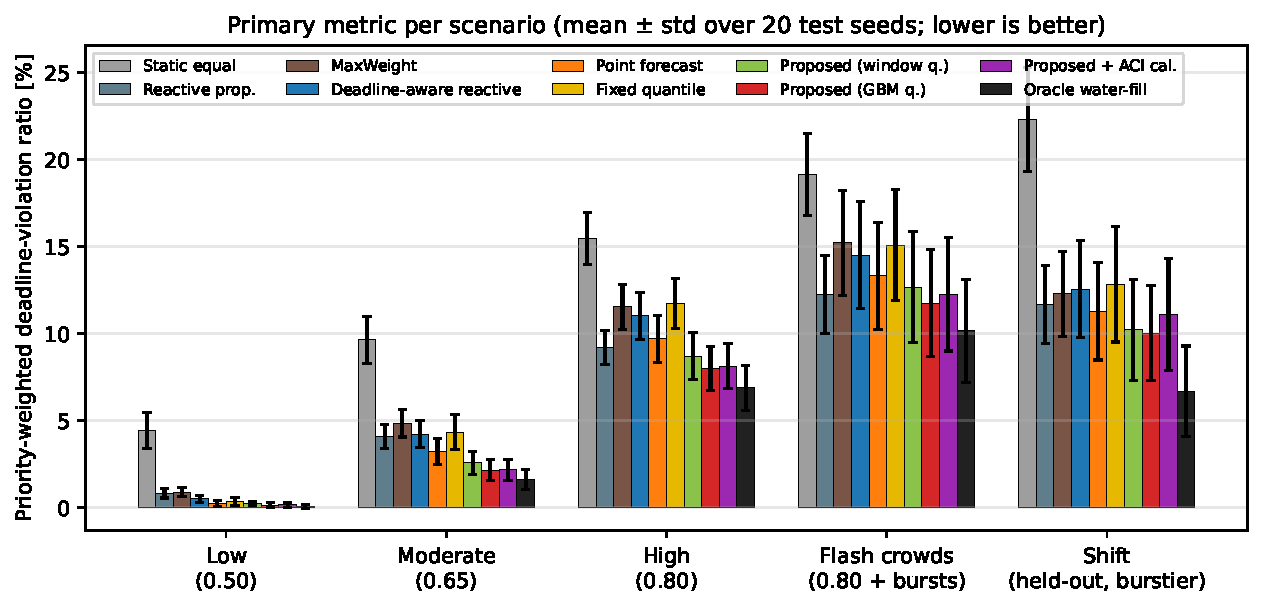
\includegraphics[width=0.95\textwidth]{fig1_primary_by_scenario.pdf}
\caption{Primary metric per scenario and controller (mean $\pm$ std over \nSeeds{} test seeds). The standard deviation across seeds is dominated by burst timing, which all controllers share seed by seed; Table~\ref{tab:paired} gives the paired reading.}
\label{fig:primary}
\end{figure*}

\subsection{Where the gain comes from}
Fig.~\ref{fig:class} decomposes the high-load scenario by class. The deadline-unaware controllers keep eMBB nearly clean (\meanhighreactivepropEMBB{}\,\% violations for reactive proportional) but let the LL cells lose \meanhighreactivepropLL{}\,\% of their bits. All deadline-aware controllers protect the LL cells (\meanhighproposedLL{}\,\% for the proposed rule) and pay with eMBB; within that group the proposed rule has the lowest eMBB loss (\meanhighproposedEMBB{}\,\% against \meanhighpointforecastEMBB{}\,\% for the point forecast) and the highest utilisation (\meanhighproposedUtil{}\,\%), because it adds margin only where the forecast is uncertain. Even the oracle loses \meanhighoracleEMBB{}\,\% of eMBB bits at 0.80 load: budgets held for 10~ms cannot follow heavy-tailed bursts, which motivates the interval study below. Jain's fairness index of per-cell service ratios exceeds 0.98 for all controllers (0.99 for all but the fixed-quantile controller), so fairness does not separate them.

\begin{figure*}[t]
\centering
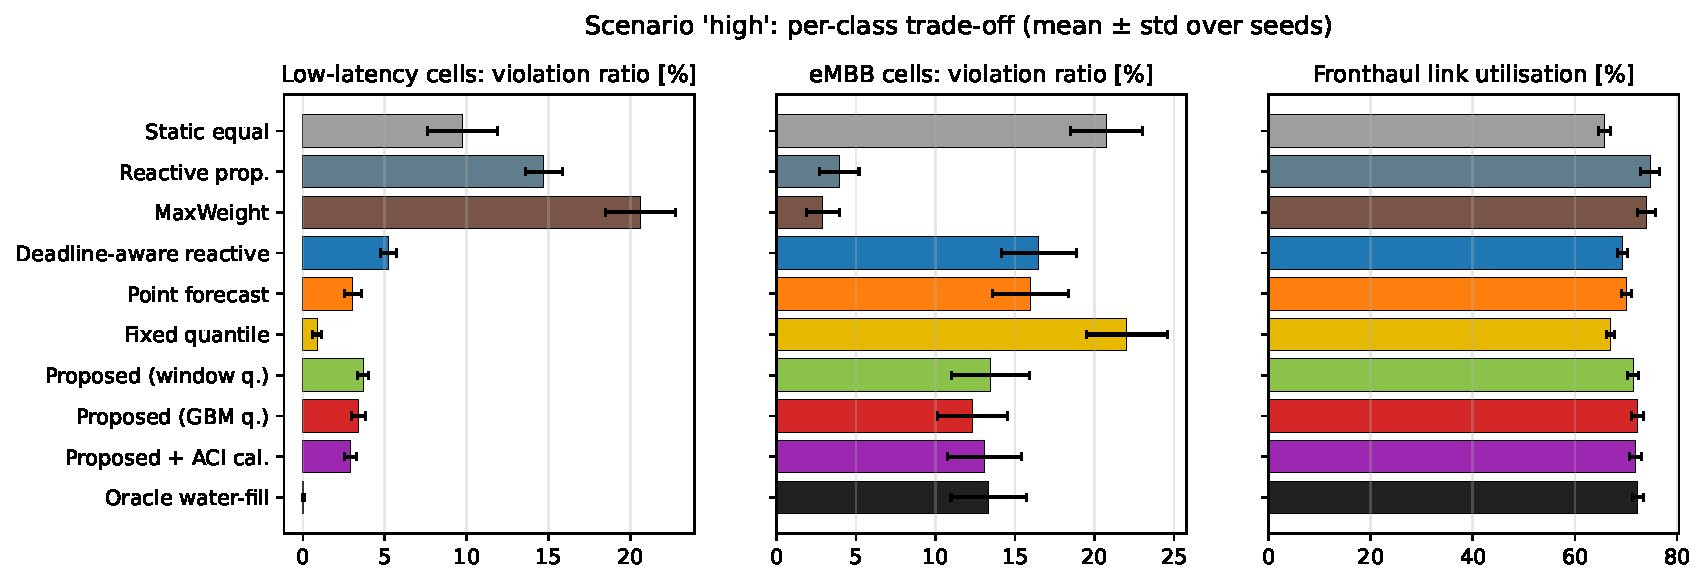
\includegraphics[width=0.95\textwidth]{fig2_class_breakdown_high.pdf}
\caption{High-load scenario: violation ratio of LL cells, of eMBB cells, and link utilisation (mean $\pm$ std over seeds).}
\label{fig:class}
\end{figure*}

\subsection{Ablations}
\textbf{Distribution versus point.} Replacing the quantile forecast by its median under the same rule family costs \redPFmin{}--\redPFmax{}\,\% (Table~\ref{tab:paired}).
\textbf{Learned versus empirical quantiles.} The same KKT rule fed with empirical window quantiles is already better than every baseline; the learned model adds a further \redshiftproposedwindow{}\,\% under the held-out shift and up to \redlowproposedwindow{}\,\% in the nominal family. Most of the gain therefore comes from the demand notion and the rule, not from the learning, and the non-learned variant is a credible fallback.
\textbf{Online conformal calibration} did not help: it is \redhighproposedcal{}\,\% worse at high load and \redshiftproposedcal{}\,\% worse under shift. In a coupled allocation the LL misses are partly caused by the shortage split rather than by forecast bias, so the per-cell correction inflates LL reservations and starves eMBB. Per-stream conformal correction \cite{cohen2023} does not transfer directly to coupled allocation; a correction acting on $\lambda$ or on unconstrained forecast error is future work.

\subsection{Control interval}
Table~\ref{tab:sweep} varies $T$ with forecasters retrained per interval (\nSeedsSweep{} seeds, scenario high). At $T = 2$~ms the proposed rule reduces $V_w$ by \sweepTfouroracle{}\,\% even relative to the oracle water-fill, which has a perfect point forecast: the allocation rule, not only the forecast, carries the gain, and the oracle is a reference rather than a bound. At $T = 20$~ms, five times the LL deadline, reserving the LL peak rate for the whole interval wastes capacity and the deadline-unaware proportional controller is better (relative reduction by the proposed rule \sweepTfourzeroreactiveprop{}\,\%). The method is thus appropriate for control intervals up to a few times the shortest deadline; the 10-ms default lies inside that range.

\begin{table}[t]
\caption{Control-interval sweep, scenario high: $V_w$ (\%, mean over \nSeedsSweep{} seeds)}
\label{tab:sweep}
\centering
\footnotesize
\resizebox{\columnwidth}{!}{% ---- inlined from generated/tab_sweep ----
\begin{tabular}{lcccc}
\hline
Controller $\backslash$ $T$ & 2 ms & 5 ms & 10 ms & 20 ms \\
\hline
Reactive proportional & 3.91 & 7.42 & 8.91 & 11.80 \\
Deadline-aware reactive & 7.89 & 10.20 & 10.78 & 15.84 \\
Point forecast + WF & 6.57 & 7.53 & 9.46 & 14.08 \\
\textbf{Proposed (GBM + KKT)} & 3.07 & 5.07 & 7.71 & 13.15 \\
Oracle water-fill & 6.89 & 6.01 & 6.63 & 10.83 \\
\hline
\end{tabular}
% ---- end generated/tab_sweep ----
}
\end{table}

\subsection{Telemetry delay}
Table~\ref{tab:delay} varies the staleness $\tau$ of the observed state with forecasters retrained per $\tau$ (\nSeedsDelay{} seeds, scenario high). All controllers degrade as information ages and the ordering is preserved at every $\tau$. The margin over the deadline-aware controllers is stable (\delayTauzeroqueueaware{}\,\% at $\tau = 0$ to \delayTauonezeroqueueaware{}\,\% at $\tau = 5$~ms against the deadline-aware reactive controller, \delayTauzeropointforecast{}\,\% to \delayTauonezeropointforecast{}\,\% against the point forecast), but the margin over the deadline-unaware proportional controller shrinks from \delayTauzeroreactiveprop{}\,\% to \delayTauonezeroreactiveprop{}\,\%: with state 5~ms old, more than twice the LL deadline, protecting the LL cells from a forecast costs almost as many weighted eMBB bits as it saves. Timely telemetry is therefore part of the operating regime of the method, as is a short control interval.

\begin{table}[t]
\caption{Telemetry-delay sweep, scenario high: $V_w$ (\%, mean over \nSeedsDelay{} seeds)}
\label{tab:delay}
\centering
\footnotesize
\resizebox{\columnwidth}{!}{% ---- inlined from generated/tab_delay ----
\begin{tabular}{lcccc}
\hline
Controller $\backslash$ $\tau$ & 0 ms & 1 ms & 2.5 ms & 5 ms \\
\hline
Reactive proportional & 8.16 & 8.91 & 9.86 & 11.30 \\
Deadline-aware reactive & 9.89 & 10.78 & 11.90 & 13.93 \\
Point forecast + WF & 8.45 & 9.46 & 10.51 & 12.45 \\
\textbf{Proposed (GBM + KKT)} & 6.85 & 7.71 & 8.77 & 11.07 \\
\hline
\end{tabular}
% ---- end generated/tab_delay ----
}
\end{table}

\subsection{Robustness to miscalibration}
\label{sec:robust}
To test Proposition~\ref{prop:robust}, every forecast quantile level is shifted by $\epsilon \in [-0.3, 0.3]$ before allocation, which moves the reported distribution by a Kolmogorov distance of $|\epsilon|$ (Table~\ref{tab:misc}, Fig.~\ref{fig:misc}). The response is asymmetric. Under-reserving ($\epsilon < 0$) is almost harmless (\mischighUnder{}\,\% at $\epsilon = -0.3$ against \mischighBase{}\,\% at $\epsilon = 0$ in the high scenario): when the link constraint binds, a common shift of all probability levels is largely absorbed by the multiplier $\lambda^\ast$, since the rule equalises weighted levels rather than using them absolutely. Over-reserving degrades gradually, to \mischighWorst{}\,\% at $\epsilon = +0.3$ (\mischighWorstRel{}\,\% relative; \miscshiftWorstRel{}\,\% under shift), because the upper quantiles saturate at the last knot and the rule loses the tail resolution that distinguishes cells. Even at the extreme the proposed rule matches the point-forecast controller (\mischighpointforecast{}\,\% at high load, \miscshiftpointforecast{}\,\% under shift) and stays below the deadline-aware reactive controller (\mischighqueueaware{}\,\%, \miscshiftqueueaware{}\,\%). The degradation is bounded and roughly linear in $\epsilon$ on the over-reserving side, consistent with Proposition~\ref{prop:robust}.

\begin{table}[t]
\caption{Forecast miscalibration: $V_w$ (\%) of the proposed rule when all quantile levels are shifted by $\epsilon$ (\nSeedsMisc{} seeds)}
\label{tab:misc}
\centering
\footnotesize
\resizebox{\columnwidth}{!}{% ---- inlined from generated/tab_misc ----
\begin{tabular}{lccccccc}
\hline
$\epsilon$ & -0.3 & -0.2 & -0.1 & +0.0 & +0.1 & +0.2 & +0.3 \\
\hline
High 0.80 & 7.80 & 7.64 & 7.61 & 7.71 & 8.13 & 9.13 & 9.45 \\
Shift & 10.96 & 10.94 & 11.10 & 11.13 & 11.53 & 12.27 & 12.50 \\
\hline
\end{tabular}
% ---- end generated/tab_misc ----
}
\end{table}

\begin{figure}[t]
\centering
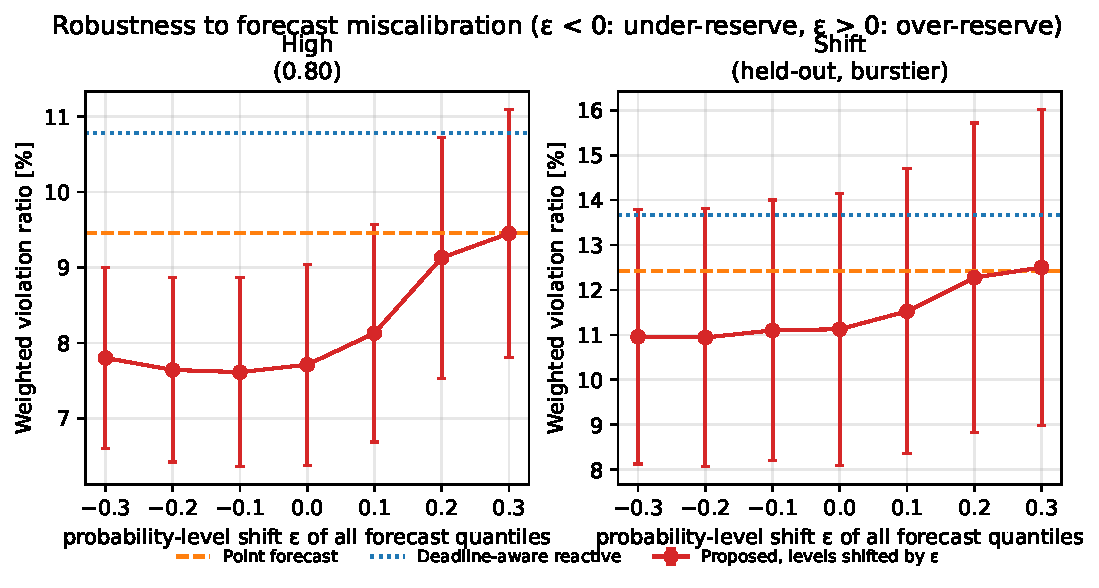
\includegraphics[width=\columnwidth]{fig10_miscalibration.pdf}
\caption{Robustness to forecast miscalibration. Dashed and dotted lines: point-forecast and deadline-aware reactive controllers on the same traces.}
\label{fig:misc}
\end{figure}

\subsection{Compression as a load lever}
\label{sec:compression}
Table~\ref{tab:compression} runs the same user traffic (moderate scenario, \nSeedsComp{} seeds) with BFP mantissa widths of 6, 9, 12 and 14 bits, which rescale $\beta$ in \eqref{eq:beta} and move the offered load from 0.44 to 0.99. At load 0.44 almost nothing is lost whatever the rule; at the default 0.65 the proposed rule loses about half as much as the reactive controllers; at 0.86 the deadline-unaware proportional controller is already slightly better on the weighted metric; at 0.99 the link is saturated and no allocation rule helps, the proposed rule being the worst because protecting the LL cells costs more eMBB bits than the priority weight repays. Compression selects the load regime; deadline-aware allocation matters most between about 0.5 and 0.8 and should hand over to pure proportional sharing, or to stronger compression, above that. The signal-quality cost of narrower mantissas is not modelled here and must be weighed against this gain in a joint design.

\begin{table}[t]
\caption{Compression width versus allocation rule, moderate scenario: $V_w$ (\%, mean over \nSeedsComp{} seeds)}
\label{tab:compression}
\centering
\footnotesize
\resizebox{\columnwidth}{!}{% ---- inlined from generated/tab_compression ----
\begin{tabular}{lcccc}
\hline
BFP mantissa bits & 6 & 9 & 12 & 14 \\
Offered load & 0.44 & 0.65 & 0.86 & 0.99 \\
\hline
Reactive proportional & 0.22 & 3.90 & 11.37 & 17.29 \\
Deadline-aware reactive & 0.18 & 4.02 & 13.84 & 20.38 \\
Point forecast + WF & 0.15 & 3.00 & 12.50 & 19.16 \\
\textbf{Proposed (GBM + KKT)} & 0.11 & 1.96 & 12.01 & 20.81 \\
\hline
\end{tabular}
% ---- end generated/tab_compression ----
}
\end{table}

\section{Discussion and Limitations}
\label{sec:limits}
The results support the hypothesis that, when budgets must be committed before the traffic is known, turning a forecast \emph{distribution} of deadline-feasible demand into per-cell budgets through the KKT rule reduces priority-weighted deadline violations compared with point forecasts, tuned global quantiles, queue-based and deadline-aware reactive controllers, including under a traffic family not seen in training. Four findings qualify the claim. First, the rule depends on the control interval being at most a few times the shortest deadline; at longer intervals interval-level reservation of a peak rate stops making sense. Second, the same holds for telemetry age: at $\tau$ beyond the LL deadline the advantage over proportional sharing nearly vanishes. Third, under sustained overload (load above about 0.85) no allocation rule helps and the problem must be solved by compression or capacity. Fourth, per-stream conformal calibration harms the coupled allocation.

Limitations: traffic is synthetic; the link is a budget-enforced pipe without a switch queue or receive-window model; each cell carries one traffic class; HARQ and uplink are not modelled; the oracle is interval-level; decision time is measured in Python; and the propositions cover feasibility, equal risk, backlog priority and miscalibration robustness, not closed-loop stability or optimality. Validation on measured per-cell PRB traces and a joint compression--allocation controller that trades signal quality for load per cell are the natural next steps.

\section{Conclusion}
We formulated budget allocation on a shared O-RAN 7-2x fronthaul link as a constrained newsvendor problem on the deadline-feasible rate of each cell, derived a closed-form KKT allocation that cuts every cell at the same priority-weighted risk, proved feasibility, equal-risk, backlog-first and miscalibration-robustness properties, and evaluated it against nine comparators on identical traces over \nSeeds{} held-out seeds with paired statistics. The rule is the best implementable controller in all five scenarios, with gains that are significant after correction and that persist under distribution shift and forecast miscalibration, and its failure regimes are identified. Code, data and scripts reproduce every number in this paper.

\begin{thebibliography}{00}
\bibitem{oran_cus} O-RAN Alliance WG4, ``Control, user and synchronization plane specification,'' O-RAN.WG4.CUS.0, 2024.
\bibitem{tr38801} 3GPP, ``Study on new radio access technology: Radio access architecture and interfaces,'' TR 38.801 V14.0.0, 2017.
\bibitem{larsen2019} L. M. P. Larsen, A. Checko, and H. L. Christiansen, ``A survey of the functional splits proposed for 5G mobile crosshaul networks,'' \emph{IEEE Commun. Surveys Tuts.}, vol. 21, no. 1, pp. 146--172, 2019.
\bibitem{perez2018} G. O. P\'erez, J. A. Hern\'andez, and D. Larrabeiti, ``Fronthaul network modeling and dimensioning meeting ultra-low latency requirements for 5G,'' \emph{J. Opt. Commun. Netw.}, vol. 10, no. 6, pp. 573--581, 2018.
\bibitem{perez2019} G. O. P\'erez, D. Larrabeiti, and J. A. Hern\'andez, ``5G new radio fronthaul network design for eCPRI-IEEE 802.1CM and extreme latency percentiles,'' \emph{IEEE Access}, vol. 7, pp. 82218--82230, 2019.
\bibitem{wang2017} L. Wang and S. Zhou, ``On the fronthaul statistical multiplexing gain,'' \emph{IEEE Commun. Lett.}, vol. 21, no. 5, pp. 1099--1102, 2017.
\bibitem{lagen2022} S. Lag\'en, X. Gelabert, A. Hansson, M. Requena, and L. Giupponi, ``Fronthaul compression control for shared fronthaul access networks,'' \emph{IEEE Commun. Mag.}, vol. 60, no. 4, pp. 70--76, 2022.
\bibitem{bega2019} D. Bega, M. Gramaglia, M. Fiore, A. Banchs, and X. Costa-P\'erez, ``DeepCog: Cognitive network management in sliced 5G networks with deep learning,'' in \emph{Proc. IEEE INFOCOM}, 2019.
\bibitem{bega2020} D. Bega, M. Gramaglia, M. Fiore, A. Banchs, and X. Costa-P\'erez, ``AZTEC: Anticipatory capacity allocation for zero-touch network slicing,'' in \emph{Proc. IEEE INFOCOM}, 2020.
\bibitem{sciancalepore2017} V. Sciancalepore, K. Samdanis, X. Costa-P\'erez, D. Bega, M. Gramaglia, and A. Banchs, ``Mobile traffic forecasting for maximizing 5G network slicing resource utilization,'' in \emph{Proc. IEEE INFOCOM}, 2017.
\bibitem{mikaeil2018} A. M. Mikaeil, W. Hu, and S. B. Hussain, ``Traffic-estimation-based low-latency XGS-PON mobile front-haul for small-cell C-RAN based on an adaptive learning neural network,'' \emph{Applied Sciences}, vol. 8, no. 7, p. 1097, 2018.
\bibitem{kavehmadavani2023} F. Kavehmadavani, V.-D. Nguyen, T. X. Vu, and S. Chatzinotas, ``Intelligent traffic steering in beyond 5G open RAN based on LSTM traffic prediction,'' \emph{IEEE Trans. Wireless Commun.}, vol. 22, no. 11, pp. 7727--7742, 2023.
\bibitem{kasuluru2024} V. Kasuluru, L. Blanco, C. J. Vaca-Rubio, and E. Zeydan, ``On the impact of PRB load uncertainty forecasting for sustainable open RAN,'' arXiv:2407.14400, 2024.
\bibitem{cohen2023} K. M. Cohen, S. Park, O. Simeone, P. Popovski, and S. Shamai, ``Guaranteed dynamic scheduling of ultra-reliable low-latency traffic via conformal prediction,'' \emph{IEEE Wireless Commun. Lett.}, vol. 12, no. 2, pp. 296--300, 2023.
\bibitem{gibbs2021} I. Gibbs and E. Cand\`es, ``Adaptive conformal inference under distribution shift,'' in \emph{Proc. NeurIPS}, 2021.
\bibitem{neely2010} M. J. Neely, \emph{Stochastic Network Optimization with Application to Communication and Queueing Systems}. Morgan \& Claypool, 2010.
\bibitem{hadley1963} G. Hadley and T. M. Whitin, \emph{Analysis of Inventory Systems}. Englewood Cliffs, NJ: Prentice-Hall, 1963.
\bibitem{leboudec2001} J.-Y. Le Boudec and P. Thiran, \emph{Network Calculus: A Theory of Deterministic Queuing Systems for the Internet}. Springer, 2001.
\bibitem{willinger1997} W. Willinger, M. S. Taqqu, R. Sherman, and D. V. Wilson, ``Self-similarity through high-variability: Statistical analysis of Ethernet LAN traffic at the source level,'' \emph{IEEE/ACM Trans. Netw.}, vol. 5, no. 1, pp. 71--86, 1997.
\bibitem{eckart1936} C. Eckart and G. Young, ``The approximation of one matrix by another of lower rank,'' \emph{Psychometrika}, vol. 1, no. 3, pp. 211--218, 1936.
\bibitem{halko2011} N. Halko, P.-G. Martinsson, and J. A. Tropp, ``Finding structure with randomness: Probabilistic algorithms for constructing approximate matrix decompositions,'' \emph{SIAM Review}, vol. 53, no. 2, pp. 217--288, 2011.
\end{thebibliography}

\end{document}
